
Le graphique suivant (Fig.\ref{graph3D}), repr�sentant l'application $\mathcal{W}(a;b)$ appliqu�e en la fonction (ou signal en 1D) $f=\Pi$ (d�finie dans la premi�re section de ce dossier) et utilisant l'ondelette m�re de Morlet (d�finie plus haut), illustre la richesse de la transformation en ondelettes continue. \\
A partir d'une ondelette m�re, on peut cr�er une pluralit� d'ondelettes "filles" qui vont fournir, par rapport � la transformation classique de Fourier, une plus grande pr�cision dans le traitement des signaux de fr�quences constamment changeantes.

\begin{figure}[h]
\centering
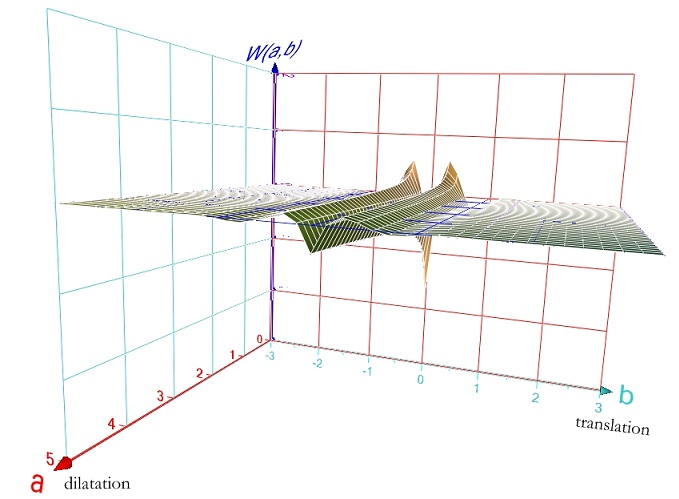
\includegraphics[scale=0.6]{images/graphe3D.jpg}
\caption{Le graphe de la fonction $\mathcal{W}(a;b)(\Pi)$}
\label{graph3D}
\end{figure}

